\chapter{Issue Tracking \\
  \small{\textit{-- Evan Ciok, Sophia DiCuffa, Carson McManus, Cindy Lee}}
  \index{Chapter!issue-tracking}
  \label{Chapter::IssueTracking}}

\section{GitHub Project}

Issue tracking and task delegation was done through GitHub Projects. Team members were able to assign tasks to themselves, as well as assign tasks to others. Team members could also mark the status of a task as ToDo, In Progress, and Done.

\begin{figure}[!htb]
    \centering
    \scalebox{0.55}{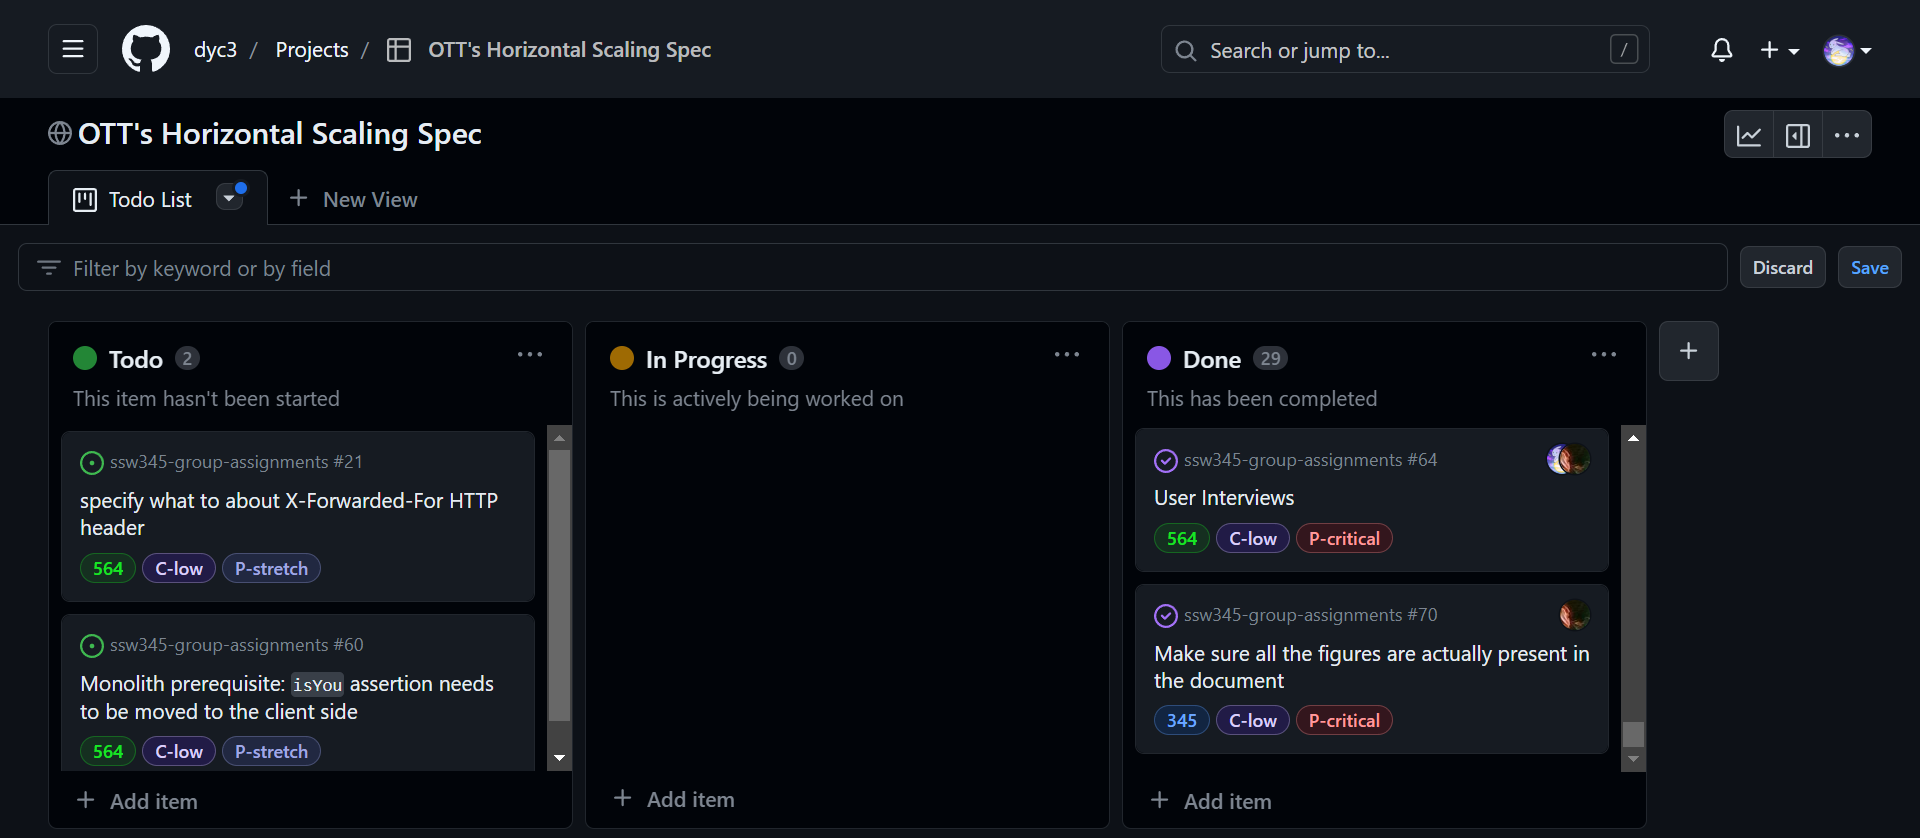
\includegraphics{Figures/github-project.png}}
    \caption{\label{Figure::github-project} Issue Tracking and Task Board in GitHub Project.}
  \end{figure}

\section{Requirements Management}

Requirements management was also done through the aforementioned GitHub Project. Individual requirements were marked as issues in GitHub, which would then become a task in the Project page.